\chapter{Results}
\label{chap:results}

Now that we have a few methods for getting the eigenvalues of the Orr-Sommerfeld equation, we can move on to calculating some results for stability. This chapter begins by showing the basic spectra we get for both Poiseuille and Couette flow, before moving on to showing the differences between each of our $ 3$ methods. We will conclude by showing that this method can be used to easily compute the eigenfunction of a flow, and by computing a numerical bound on $ R$ to compare to the analytic bounds found by Synge and Joseph that we derived back in Chapter \ref{chap:suffcons}. From this bound, we get a value for the famous critical Reynolds number for plane Poiseuille flow.

Our method is implemented in the class Appendix \ref{code:chebyshevclass}, with the matrices for each of our methods implemented in Appendix \ref{code:fourthorder}, Appendix \ref{code:secondorder} and Appendix \ref{code:firstorder}. The code for the differentiation matrices and $ P $ and $ Q $ matrices for each flow is implemented in Appendix \ref{code:tau_matrices}.

To create the spectra in the chapter we take the eigenvalues returned by our program and bound them using Josephs bounds on $ c_r$ and $ c_i$ derived in Chapter \ref{chap:suffcons}. As there is no lower bound on $ c_i$, we choose the lower bound of $ c_i = -1 $ as is the most common convention in other literature. All of our spectra contain eigenvalues with imaginary parts below $ -1 $, but any solutions related to these decay very fast and are therefore very stable. We are also much more interested in eigenvalues with imaginary parts close to zero so it makes little sense to include eigenvalues with large negative imaginary parts.

Note: Unless mentioned otherwise, the programs in this chapter were run with $ \alpha = 1$.

\section{Basic results - Poiseuille Flow}

To plot a spectrum of eigenvalues, we will plot the real part $c_r$ along the $x$-axis and the imaginary part $c_i$ along the $y$-axis. This produces a two-dimensional spectrum for us to analyse.

To begin let's examine how these methods can be used to determine whether a flow is stable or not. If a flow is unstable it will have an eigenvalue $ c$ that has imaginary part $ c_i > 0$. Figure \ref{fig:unstablevstableflow} shows the spectra for $ R = 1000$ and $ R = 7500$ produced using the second-order method with $ 200 $ polynomials. We can see from these that Poiseuille flow is stable for $R = 1000$ but is unstable for $ R  = 7500$.

\begin{figure}[h!]
    \centering
    \subfloat[$ R = 1000$]{
        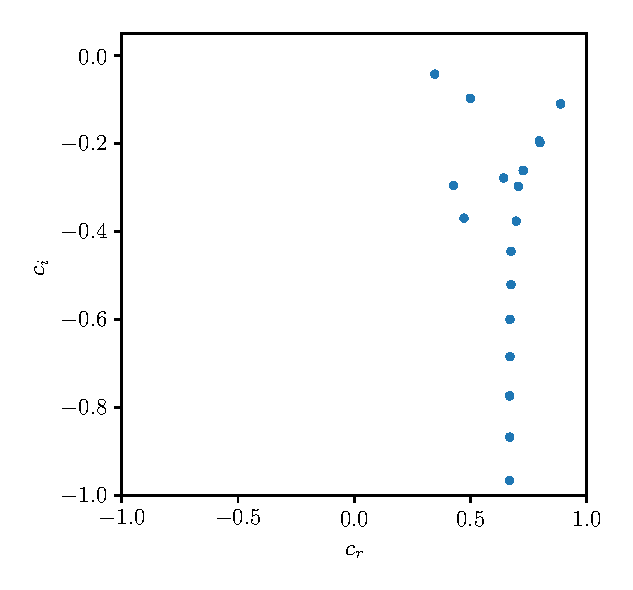
\includegraphics[width=60mm]{figures/pR=1000a=1M=200order=2.eps}
    }
    \subfloat[$ R = 7500$]{
        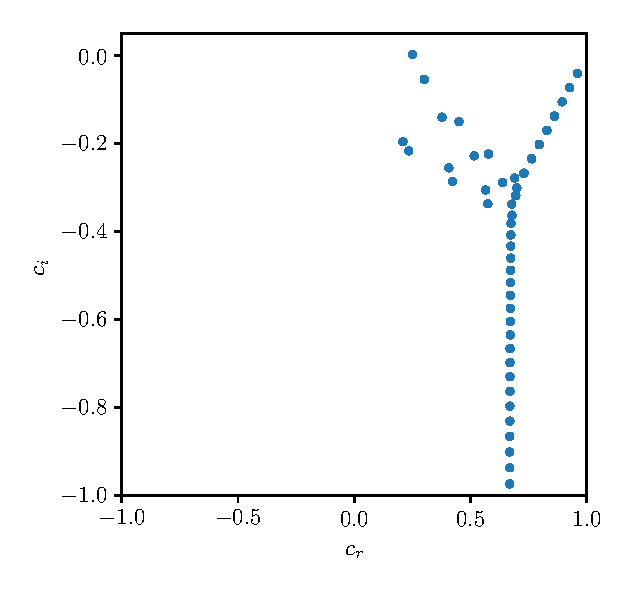
\includegraphics[width=60mm]{figures/pR=7500a=1M=200order=2.eps}
    }
    \caption{Eigenvalue spectra for a stable Poiseuille flow ($R = 1000$) and an unstable flow ($R = 7500$}
    \label{fig:unstablevstableflow}
\end{figure}

The spectrum for $ R = 10000$ and $ M = 200 $ can be seen in Figure \ref{fig:r10000} and forms a 'Y' shape. This is a classic case when it comes to Poiseuille flow and this spectrum matches those seen in papers such as \citet{dongarra1996chebyshev, bukhari1997spectral, antar1976eigenvalue}. We can see that there are 3 distinct 'families' of eigenvalues. The bottom straight line is referred to as the S family and contains a pattern of alternating odd and even eigenvalues \citep{dongarra1996chebyshev}, the top right branch is referred to as the P family and consists of overlapping pairs of odd and even eigenvalues \citep{dongarra1996chebyshev} and the 'spray' of eigenvalues forming the left branch is referred to as the A family of eigenvalues. These names come from \citet{mack1976numerical}.

\begin{figure}[h!]
    \centering
    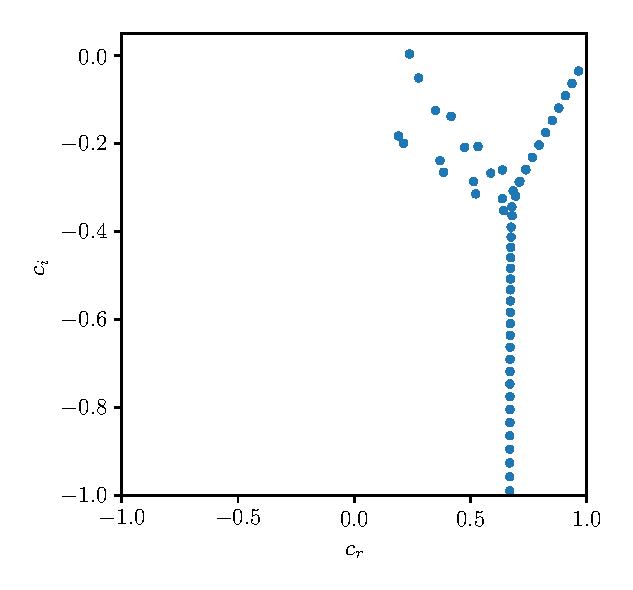
\includegraphics[width=80mm]{figures/pR=10000a=1M=200order=2.eps}
    \caption{Eigenvalue spectra for plane Poiseuille flow with $ R = 10000 $}
    \label{fig:r10000}
\end{figure}

We can see that Poiseuille flow is unstable at $ R = 10000$ because there is one 'critical eigenvalue' that has an imaginary part just slightly above $ 0 $. This is consistent with what other papers have found, most notably \citet{orszag1971accurate}. We will discuss how accurately the different methods reproduce the value of this critical eigenvalue in Section \ref{section:p_comparison}.

Finally, we should verify that all three of our methods produce similar results. Figure \ref{fig:comparison_poiseuille} shows a comparison between all three methods for Poiseuille flow at $ \al = 1 $, $ R = 10000 $ with $ 200 $ polynomials ($ M = 200$). As can be seen, the spectra all look similar, showing that the methods appear to be consistent. However, there are significant differences between these methods which can become more pronounced at higher and lower values of $ R $ and $ M $. A more thorough comparison is the focus of Section \ref{section:p_comparison}.

\begin{figure}[h!]
    \centering
    \subfloat[Fourth order spectrum]{
        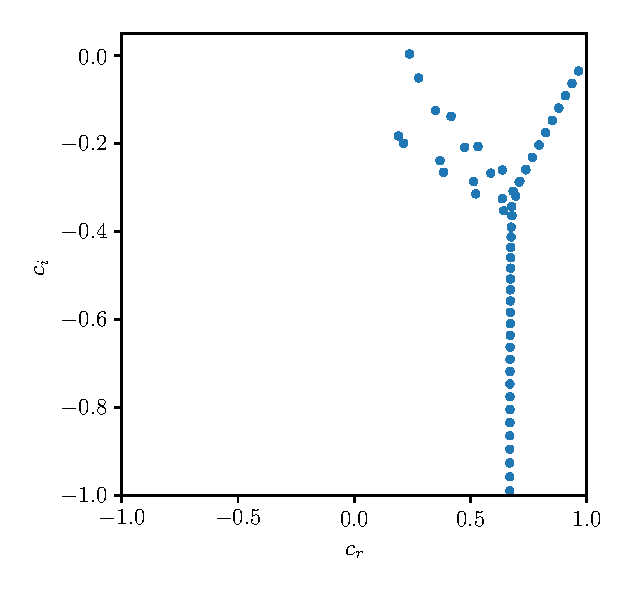
\includegraphics[width=50mm]{figures/p_flow_order_4_10000.eps}
    }
    \subfloat[Second order spectrum]{
        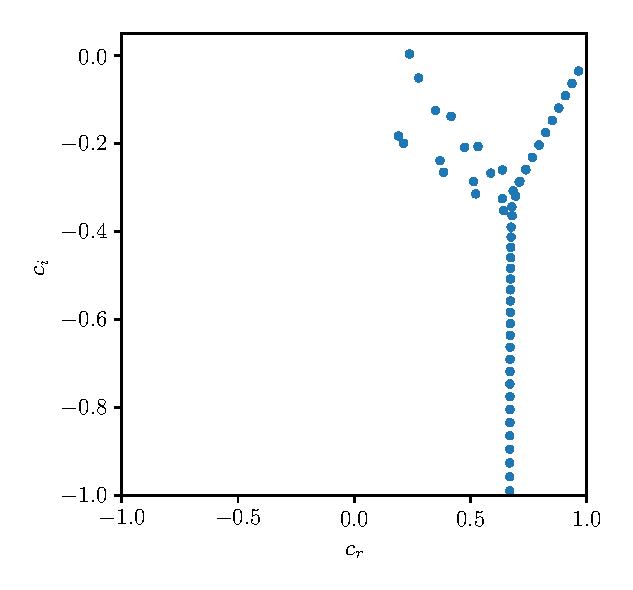
\includegraphics[width=50mm]{figures/p_flow_order_2_10000.eps} 
    }
    \subfloat[First order spectrum]{
        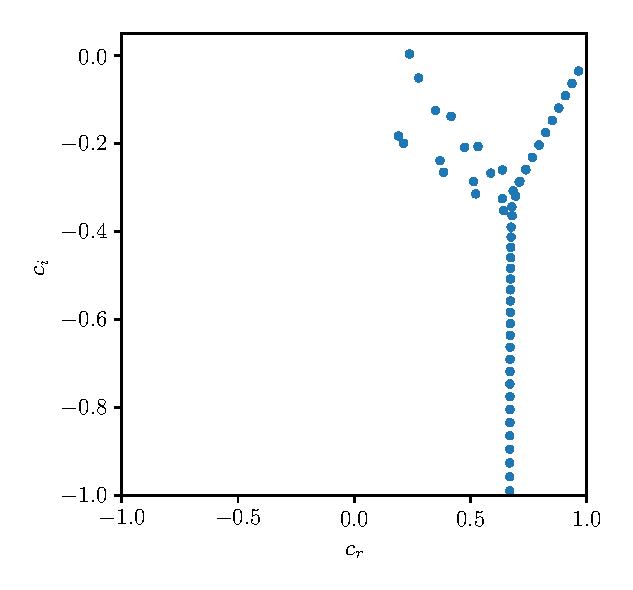
\includegraphics[width=50mm]{figures/p_flow_order_1_10000.eps}
    }
    \caption{The spectrum of Poiseuille flow for $ \al = 1 $, $ R = 10000 $ using different orders of method. They are consistent with each other which implies that these methods all work well for this value of $ R $.}
    \label{fig:comparison_poiseuille}
\end{figure}

\section{Basic results - Couette Flow}

If we run the second order method for Couette flow with $R = 8000$, $M = 200$ we get the spectrum shown in Figure \ref{fig:couettebroken}. However there is an obvious discrepancy in the spectrum when compared to the one in papers such as \citet{bukhari1997spectral}, the spectrum is not symmetric. 

\begin{figure}[h!]
    \centering
    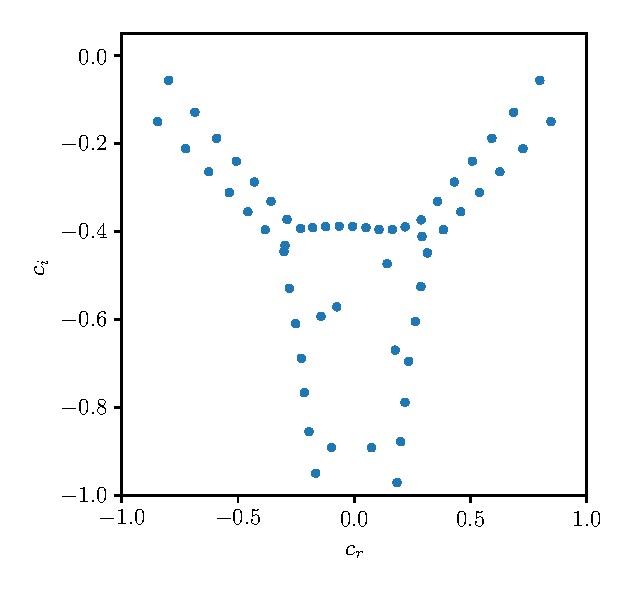
\includegraphics[width=80mm]{figures/couette_broken.eps}
    \caption{Spectrum of Couette flow with $ R = 8000$. There are some interesting discrepancies in this spectrum}
    \label{fig:couettebroken}
\end{figure}

It turns out this is due to the boundary conditions we have used causing numerical error. As noted in \citet{canuto2007spectral} in the case of plane channel flow, the odd and even terms in the sums representing our boundary conditions can be decoupled. This leaves us with an alternative set of boundary conditions
\begin{equation}
    \sum^M_{\substack{k = 0 \\ k \equiv 0 \ (\text{mod } 2)}} a_k =  \sum^M_{\substack{k = 1 \\ k \equiv 1 \ (\text{mod } 2)}} a_k = \sum^M_{\substack{k = 0 \\ k \equiv 0 \ (\text{mod } 2)}} k^2 a_k = \sum^M_{\substack{k = 1 \\ k \equiv 1 \ (\text{mod } 2)}} k^2 a_k = 0.  
\end{equation}

The first two conditions here correspond to the boundary conditions on $ \p(z)$, while the second two correspond to the boundary conditions on $ \p'(z) $. Using these alternative boundary conditions again with $ R = 8000$, $ M = 200 $ produces the spectrum seen in Figure \ref{fig:couette_fixed}. As can be seen, the result is now symmetric which fits the spectra seen in other literature such as \citet{bukhari1997spectral, DONGARRA1996399}.

The reason why these boundary conditions fix the spectrum is a little unclear. The most likely is due to the very large range in values in the matrices caused by the $ (-1)^k k^2$ in the original boundary conditions causing additional numerical error.

\begin{figure}[h!]
    \centering
    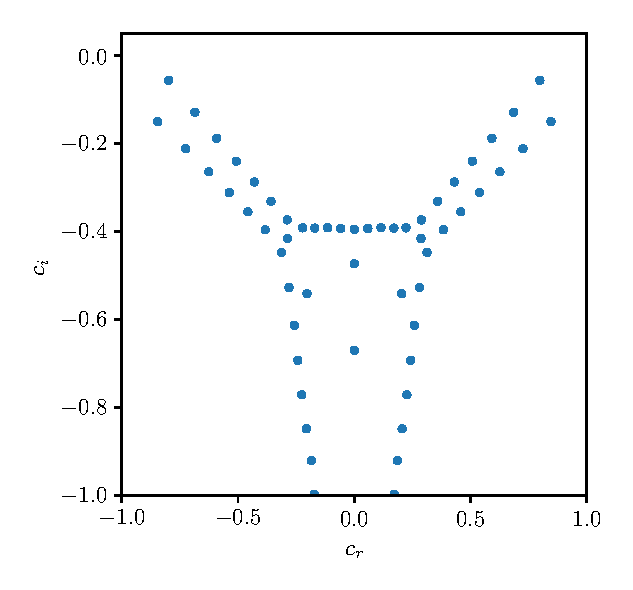
\includegraphics[width=80mm]{figures/couette_fixed.eps}
    \caption{Spectrum for Couette flow with $ R = 8000$ with alternative boundary conditions. The discrepancies seen in Figure \ref{fig:couettebroken} are not present here} 
    \label{fig:couette_fixed}
\end{figure}

If we look at Figure \ref{fig:couette_fixed}, we can see that Couette flow appears to be stable for this value of $ R$. If we test other values of $ R$ too, we find that Couette flow is stable for all values of $R$. This matches the findings of \citet{bukhari1997spectral} and other literature.

It turns out that these methods only work for very low $ R$ in the case of Couette flow. As seen in \citet{dongarra1996chebyshev}, all Couette flow spectra should look similar to the spectrum shown in Figure \ref{subfig:couette_3000}, with a single straight tail at around $ c_r = 0 $ that splits two symmetric sprays of eigenvalues as $ c_i \to 0 $. \citet{DONGARRA1996399} observed divergence from this spectrum as early as $ R = 3500 $, which our program reproduces as seen Figure \ref{subfig:couette_3500}.

\begin{figure}[h!]
    \centering
    \subfloat[$R = 3000$, $ M = 200$]{
        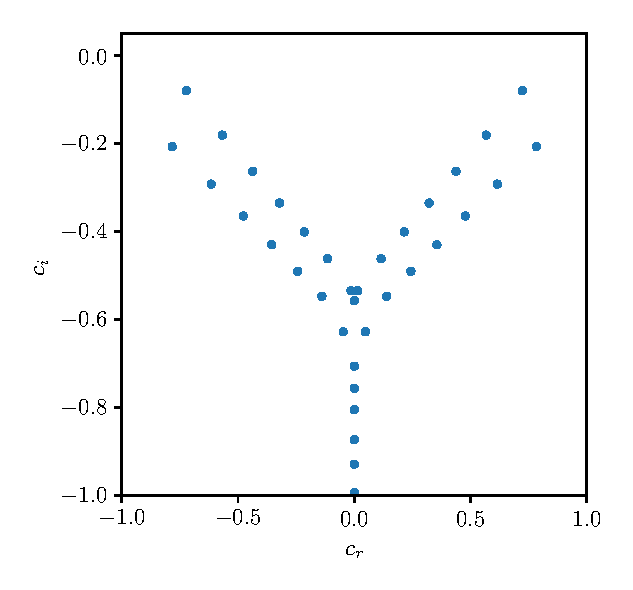
\includegraphics[width=60mm]{figures/couetteR=3000.eps} \label{subfig:couette_3000}
    }
    \subfloat[$R = 3500$, $ M = 200$]{
        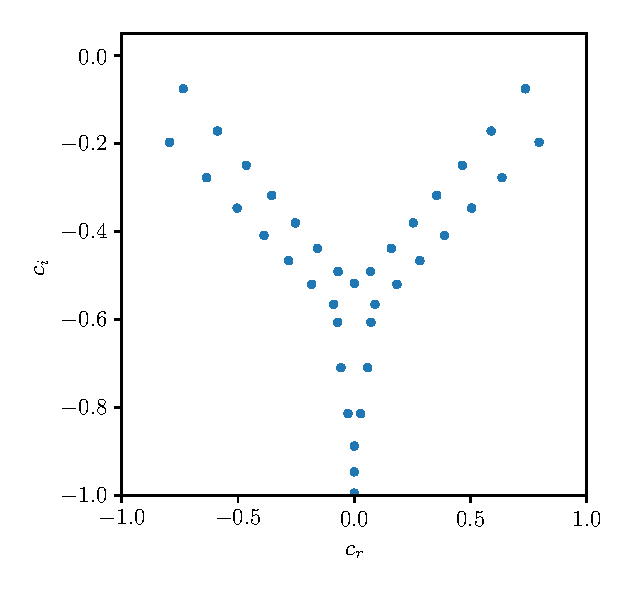
\includegraphics[width=60mm]{figures/couetteR=3500.eps} \label{subfig:couette_3500}
    }
    \caption{The spectrum of Couette flow with different values of $ R$. The left plot shows an expected plot, while the right plot shows a divergence from the expected spectrum.}
    \label{fig:couette_3000}
\end{figure}

A comparison between our three methods for Couette flow with $ R = 3000 $ with $ M = 200 $ is shown in Figure \ref{fig:comparison_couette}. As can be seen, unlike in the case of Poiseuille flow, the spectra produced vary significantly. The first order method looks the most accurate to the plot of $ R = 3000 $ in \citet{DONGARRA1996399} as expected, with the second order method looking extremely similar. On the other hand, the fourth-order method shows a significant divergence from the expected spectrum. This implies that the fourth-order method is not very good in the case of Couette flow.

\begin{figure}[h!]
    \centering
    \subfloat[Fourth order spectrum]{
        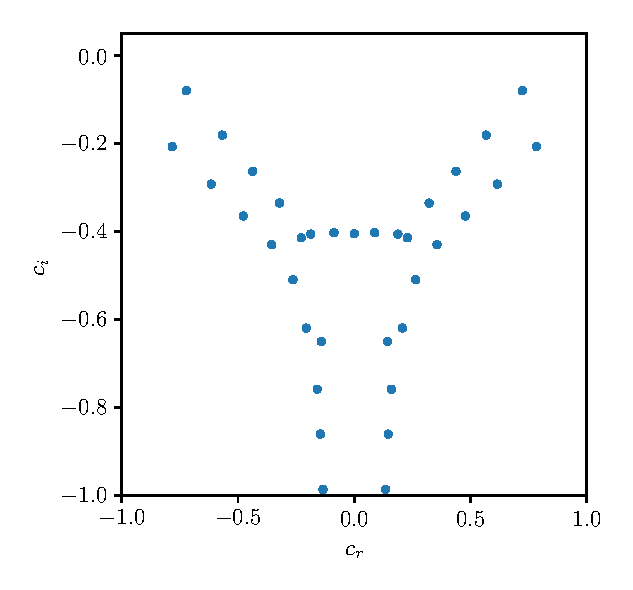
\includegraphics[width=50mm]{figures/c_flow_order_4_3000.eps}
    }
    \subfloat[Second order spectrum]{
        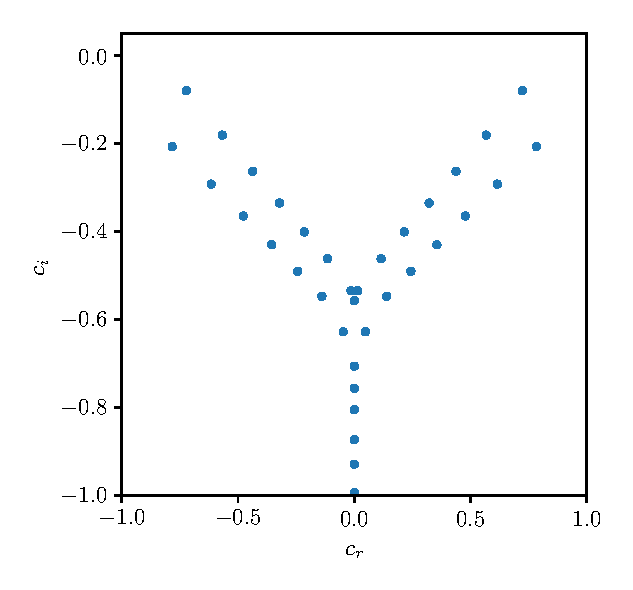
\includegraphics[width=50mm]{figures/c_flow_order_2_3000.eps} 
    }
    \subfloat[First order spectrum]{
        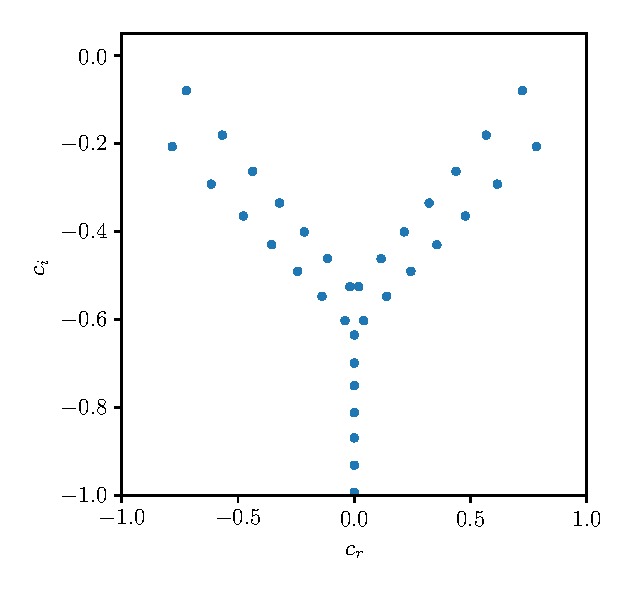
\includegraphics[width=50mm]{figures/c_flow_order_1_3000.eps}
    }
    \caption{The spectrum of Couette flow for $ R = 3000 $ using different orders of method. The fourth-order plot is significantly more diverged than the others, while the first-order method appears to be the most accurate.}
    \label{fig:comparison_couette}
\end{figure}

\citet{DONGARRA1996399} was able to get an accurate spectrum up until $ R = 13000$ by using $128$-bit floating point arithmetic rather than the $ 64$-bit arithmetic that our program uses. We can also reduce the divergence by tweaking the number of polynomials used. We will discuss this further in the next section where we compare the three different methods and their accuracy.

\section{Time Comparison of Methods} \label{section:time_comparison}

Now that we have verified the basic results of our program for both Poiseuille and Couette flow, we can move on to discussing how the $3$ different methods differ. There are advantages and disadvantages to each, so is there an obviously best choice? 

To start with let's compare perhaps the most obvious difference that we notice when running these programs, the difference in computation time. As mentioned in Chapter \ref{chap:numerics}, each method requires larger and larger matrices, and therefore more operations to both set up and solve. The Python program in Appendix \ref{code:timecomp} calculates the time taken for each method for different values of $M $. Figure \ref{fig:timecomp} shows the results of this program, a time comparison between the fourth-order method (green line), second-order method (orange line) and first-order method (blue line) for various values of $M$. 

As we can see there is a significant difference in the time taken for each of the methods, particularly between the first-order method and the other two methods. Even using just $ M = 200$ the first order method is significantly slower than the other two - taking over $2$ minutes to run at $M = 500$! This graph also highlights the main advantage of the fourth-order method, its speed. Notice also that while slower than the fourth order method, the second order method is still much faster than the first order method, taking less than $20$ seconds at $M = 500$. 

\begin{figure}
    \centering
    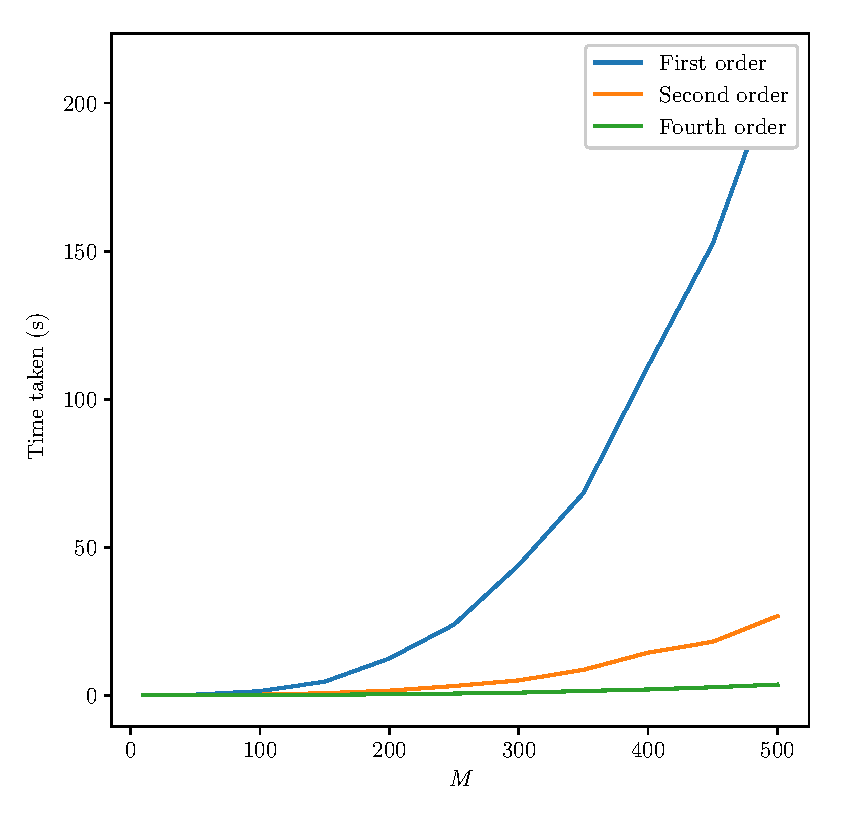
\includegraphics[width=100mm]{figures/time_comparison.eps}
    \caption{A comparison of times for the methods of different orders.}
    \label{fig:timecomp}
\end{figure}

So if the fourth-order method is that much faster than the other two methods, why bother using the others at all? The answer is due to the amount of accuracy that is lost at higher values of $ M $ or even $ R$. As we will see, each method of decreasing order is more accurate than the one before. But how does this inaccuracy present itself in the cases of Poiseuille and Couette flow? 

\section{Accuracy - Poiseuille Flow} \label{section:p_comparison}

To start with let's examine these methods in the case of Poiseuille flow. Figure \ref{fig:inaccdemo} shows eigenvalue spectra for the second order method run for $ R = 20000 $ with $ M = 150,\ 200,\ \text{and } 1000 $. The $ M = 200 $ plot looks as we would expect, but we see some interesting features in the $M = 150 $ and $ M = 1000 $ plot. 

\begin{figure}[h!]
    \centering
    \subfloat[$R = 20000,\ M = 150 $]{
        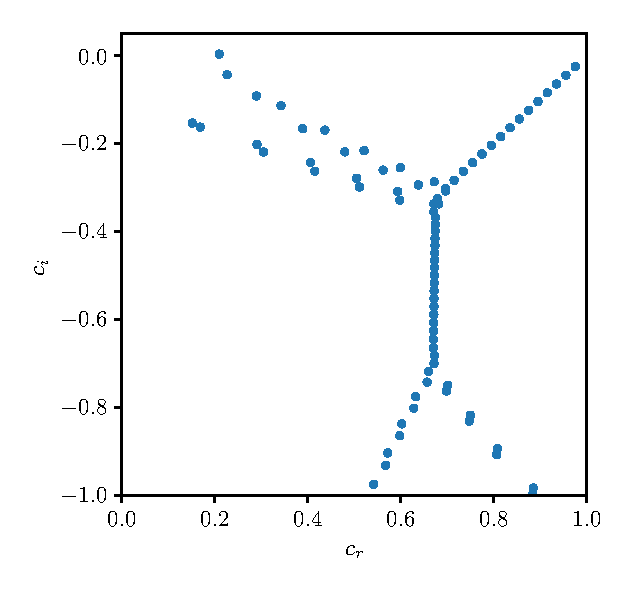
\includegraphics[width=50mm]{figures/pR=20000a=1M=150order=2.eps}
    }
    \subfloat[$R = 20000,\ M = 200 $]{
        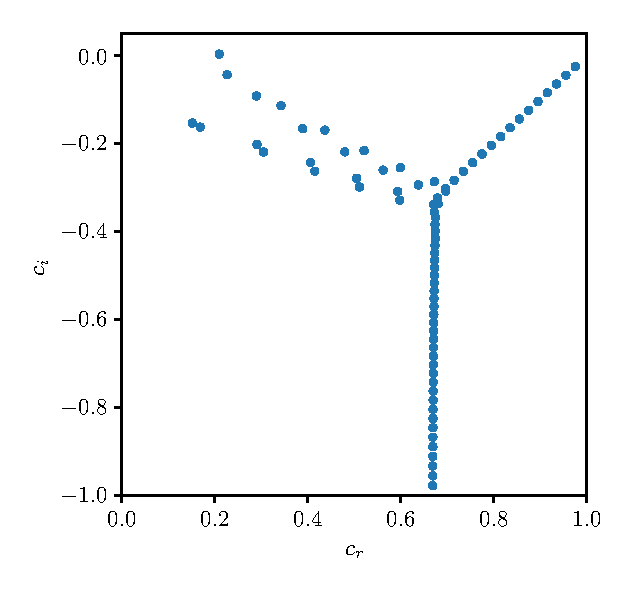
\includegraphics[width=50mm]{figures/pR=20000a=1M=200order=2.eps}
    }
    \subfloat[$R = 20000,\ M = 1000 $]{
        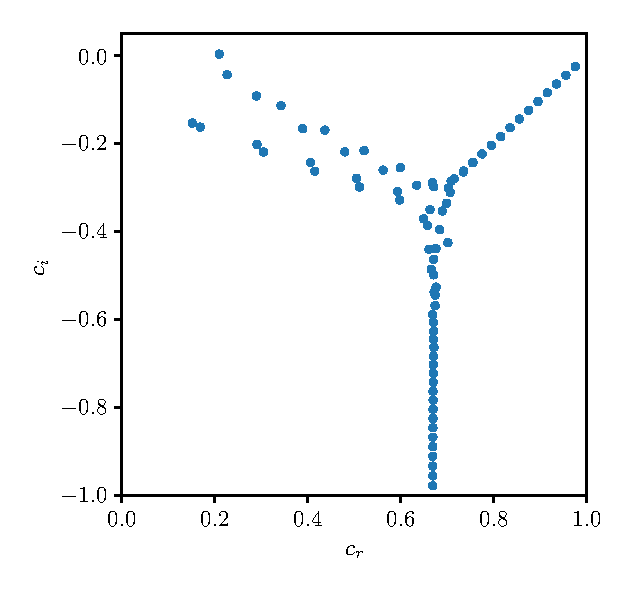
\includegraphics[width=50mm]{figures/pR=20000a=1M=1000order=2.eps}
    }
    \caption{Eigenvalue spectra for various values of $ M $ with $ R = 20000 $}
    \label{fig:inaccdemo}
\end{figure}

In the $M = 150 $ plot we can see a 'split' in the S family of eigenvalues. This tail is caused by using a number of polynomials that is too low to accurately determine eigenvalues with a lower imaginary part \citep{dongarra1996chebyshev}. In fact, if we extended the graph down on the $ M = 200$ and $M = 1000$ plots we would see a similar split. The reason that this isn't a concern is that we are concerned with the stability of the solution, and therefore care more about eigenvalues with imaginary parts that are close to $ 0$. The modes with eigenvalues with imaginary parts much below $0$ decay extremely fast and therefore are very stable.  

If we look at the $ M = 1000$ plot we can see a small triangle in the centre of the spectra, where the $3 $ branches meet. This is sometimes referred to as the 'triangle of instability' and is an indication that numerical error is present in the spectra \citep{dongarra1996chebyshev}. This occurs when either $ R$ or $ M $ is too high. We can use this to easily visualise the difference in numerical error between our different methods. Figure \ref{fig:trianglecomp} shows the spectra for $ R = 30000$ with $ M = 500$ generated by the fourth-order, second order and first-order methods respectively.

\begin{figure}[h!]
    \centering
    \subfloat[Fourth order]{
        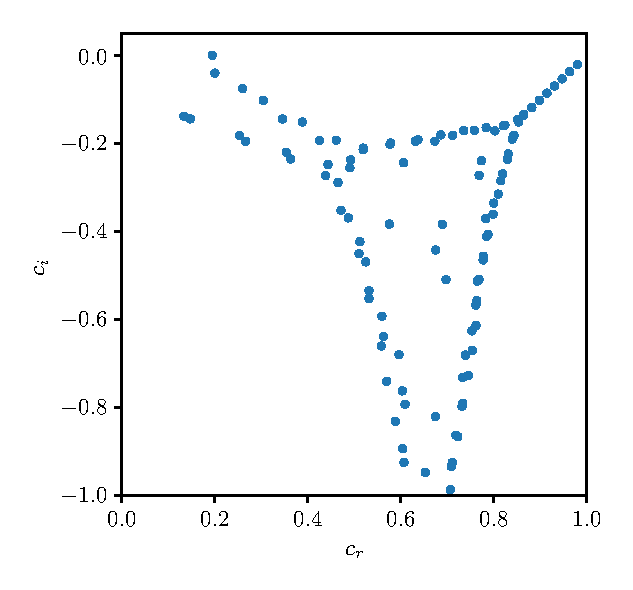
\includegraphics[width=50mm]{figures/pR=30000a=1M=500order=4.eps}
    }
    \subfloat[Second order]{
        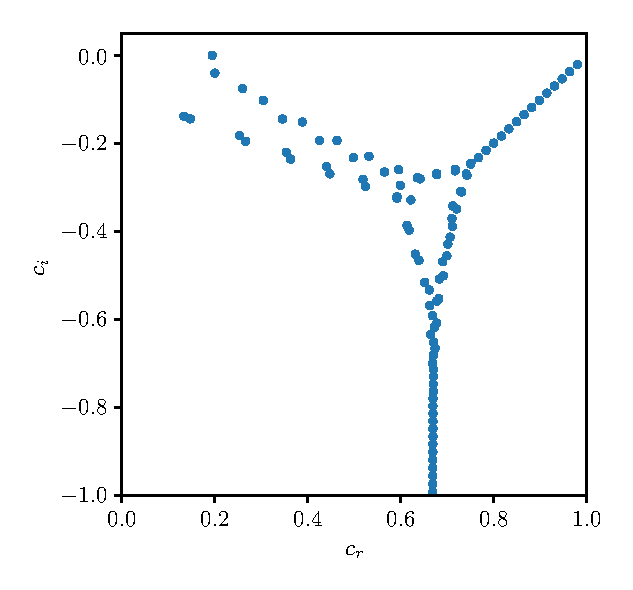
\includegraphics[width=50mm]{figures/pR=30000a=1M=500order=2.eps}
    }
    \subfloat[First order]{
        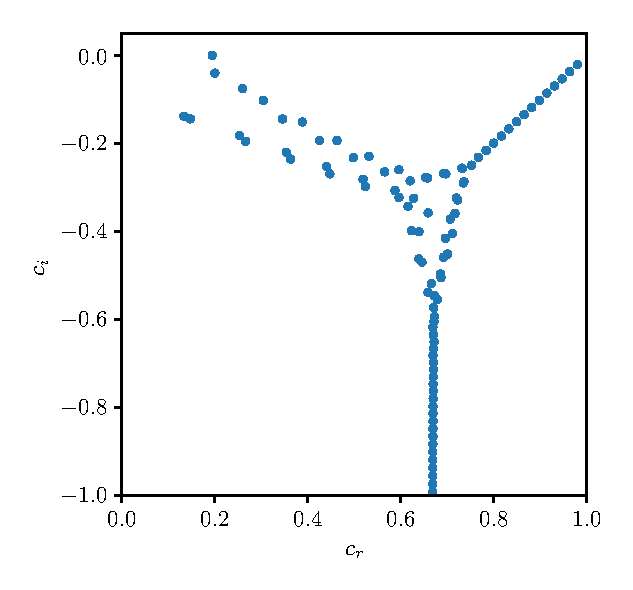
\includegraphics[width=50mm]{figures/pR=30000a=1M=500order=1.eps}
    }
    \caption{Eigenvalue spectra for $ R = 30000$, $ M = 500$ generated using methods of decreasing order (left to right)}
    \label{fig:trianglecomp}
\end{figure}

As can be seen, the difference in numerical accuracy between the fourth-order method (left spectrum) and second-order method (centre spectrum) is massive, the triangle of instability heads off of the bottom of the screen in this example. However while noticeable, the plots imply that the numerical error between the second-order method (centre spectra) and the first-order method (right spectra) is far less significant. This is an extreme example however, it turns out that the triangle of numerical error can never be removed from the spectrum of $ R = 30000$ no matter how high the number of polynomials used. A solution may be to use higher precision floating points, as \citet{dongarra1996chebyshev} show in the $ R = 28000$ case this can get rid of the triangle of instability altogether. 

This along with Figure \ref{fig:inaccdemo} imply two important things about these methods. First of all, the number of polynomials (value of $M $) chosen affects the accuracy of the produced spectra significantly. This must be remembered if the aim is to get an accurate representation of a specific portion of the spectra for a given value of $ R$. Secondly, if the value of $ R $ is high enough there is no way of completely removing the numerical instability. This implies that for high values of $R$, this method is not very useful for determining the eigenvalue spectrum. 

However, there is another more important way that numerical error can present itself. This is in the accuracy of the critical eigenvalue. This value must be computed accurately as it often has an imaginary part very close to zero and if computed incorrectly we could end up drawing the wrong conclusion about the stability of a flow.

\citet{orszag1971accurate} computed the critical eigenvalue for Poiseuille flow with $R = 10000$, $ \al = 1$ and (to 8 decimal places) found a value of 
\begin{equation}
     0.23752649 + 0.00373967i.
\end{equation} 

Table \ref{table:comparison} shows a side-by-side comparison of the critical eigenvalue produced by each method at different values of $M $ for Poiseuille flow with $ R = 10000$, $ \al = 1$. We can see a few interesting things here. First, all three methods obtain the correct eigenvalue at around $ M = 60$, though the first-order method produces the value accurately slightly earlier at around $M = 50$. Secondly, as $M $ gets larger the fourth-order and second-order methods lose accuracy. The fourth-order method is only accurate to 5 decimal places by the time $M = 200$, whereas the second-order and first-order methods are still accurate to 8 decimal places. By the time $M = 500$, the fourth-order method is only accurate to 4 decimal places. At this point, the second-order method has lost some accuracy and is now only accurate to 7 decimal places, but the first-order method is still accurate to 8 decimal places. This implies that the numerical error in the first-order method has a magnitude of less than $ 10^{-8}$ at $ M = 500$. This shows that the lower-order methods are indeed more accurate, as is expected with the tau method. 

\begin{table}[h!]
\centering
 \begin{tabular}{c | c | c | c} 
 M & Fourth-order & Second-order & First-order \\ [0.5ex] 
 \hline
 10 & 0.74378020+0.63468457i & 0.94669728+0.38207669i & 0.94669728+0.38207669i \\ 
 20 & 0.73281177+0.0921027i & 0.64429837+0.06460278i & 0.64429837+0.06460278i \\
 30 & 0.23690887+0.00365516i & 0.23757258+0.00374383i & 0.23747672+0.00364734i \\
 40 & 0.23752676+0.00373427i & 0.23752741+0.00374191i & 0.23752761+0.00373901i \\
 50 & 0.23752651+0.00373968i & 0.23752648+0.00373967i & 0.23752649+0.00373967i \\ 
 60 & 0.23752649+0.00373967i & 0.23752649+0.00373967i & 0.23752649+0.00373967i \\
 \vdots & \vdots & \vdots & \vdots \\
 200 & 0.23752588+0.00374036i & 0.23752649+0.00373967i & 0.23752649+0.00373967i \\
 \vdots & \vdots & \vdots & \vdots \\
 500 & 0.2374707+0.00378162i & 0.23752646+0.00373950i & 0.23752649+0.00373967i \\
 \end{tabular}
 \caption{Comparison of critical eigenvalue produced by each method for $ R = 10000 $ for increasing values of $ M $. }
 \label{table:comparison}
\end{table}

Let's examine the convergence of the first-order method more closely for values above $ M = 50$. Table \ref{table:firstorder} contains the critical eigenvalues produced by the first-order method for $ M $ between 50 and 120. We can see that for $ M > 70$, the first 11 decimals are the same. As the tau method is expected to converge as $M $ increases, we can confidently say that this is a more accurate value for the critical eigenvalue for Poiseuille with $ R = 10000 $. Our estimate for the critical eigenvalue to 11 decimal places is
\begin{equation}
    0.23752648882+0.00373967062i.
\end{equation}

\begin{table}[h!]
\centering
 \begin{tabular}{c | c} 
 M & Critical Eigenvalue - First-order \\ [0.5ex] 
 \hline
 50  & 0.23752648798891834+0.0037396745437875040i \\
 60  & 0.23752648882528551+0.0037396706118949263i \\
 70  & 0.23752648882056760+0.0037396706231014325i \\
 80  & 0.23752648882017588+0.0037396706228313510i \\
 90  & 0.23752648882049590+0.0037396706231066680i \\  
 100 & 0.23752648882102453+0.0037396706230743916i \\
 110 & 0.23752648882018287+0.0037396706236932730i \\
 120 & 0.23752648882051130+0.0037396706231617796i 
 \end{tabular} 
 \caption{Critical eigenvalues for the first-order method. }
 \label{table:firstorder}
\end{table}

It is difficult to confirm that this is definitely the critical eigenvalue of Poiseuille flow with $ R = 10000 $ to $ 11 $ decimal places since in other literature, the authors only attempt to reproduce the $ 8 $ decimal place value found by \citet{orszag1971accurate}. Still, \citet{bukhari1997spectral} found that error was lowest at around this range of $ M $ and this value does match the value given by \citet{orszag1971accurate} to $8$ decimal places. The author of this report believes that this is a more accurate eigenvalue than that found by \citet{orszag1971accurate}.

We can also see that there appears to be a 'sweet spot' for accurately determining the critical eigenvalue for all of our methods at around $ M = 60$. This is interesting because this value of $ M $ is too low to obtain the whole spectrum correctly. This means there is a trade-off between accurately determining the critical eigenvalue for a flow compared to getting more accurate results for other eigenvalues. The more eigenvalues we try and determine, the less accurate our value for the critical eigenvalue is.

However, for high values of $R$ the numerical error in the critical eigenvalue is too high and as such we get that after a certain point, all flows are computed to be stable. This is the case no matter the method. For example, when $ R = 35000 $, all of our methods return that the flow is stable. But, we know that flows above a certain critical value of $R$ are unstable from our analytical bounds derived in Chapter \ref{chap:suffcons}. This means that since we've found that Poiseuille flow is unstable for $ R = 10000$, it must also be unstable for $ R = 35000 $, indicating that our program is incorrect. This isn't a concern, however, as we can still search for the critical value of $R$ as it must be below $ 10000$, and our methods accurately determine the stability of flows for lower $R$ values. We will compute this value in Section \ref{section:crit_r}.


% Figure \ref{fig:criterrorcomp} shows a graph of the error in the critical eigenvalue for each method for different values of $\log M $. This is specifically for the $ R = 10000 $ case. The most noticeable thing here is that the fourth-order method never determines the value of the critical eigenvalue to particularly high accuracy, whereas the second-order and first-order methods correctly compute the critical eigenvalue to around 8 decimal places. Notice also that this graph implies that there is a 'best' value for $M$, after which numerical error sets in and the computed value diverges from the true value (our approximation should converge as $ M \to \infty$).

% \textbf{make this figure nicer and explain where this error comes from. also actually compute the best number of polys to use}

% \begin{figure}
%     \centering
%     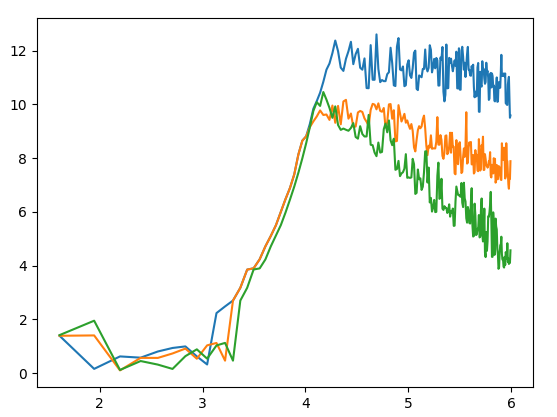
\includegraphics{figures/PlaceholderCritEigError.png}
%     \caption{Comparison of error between }
%     \label{fig:criterrorcomp}
% \end{figure}

% For both the second and first-order methods this peak occurs at around $M = 77  $, which agrees with \citet{dongarra1996chebyshev} who found that both these methods agree with the value \cite{orszag1971accurate} computed after this point. For $ R = 10000$ with $ 56 $ polynomials with both the second and first-order method, we find that the critical eigenvalue is (to $8$ decimal places)
% \begin{equation}
%     0.23752649 + 0.00373967 i,
% \end{equation}
% which agrees exactly with \citet{orszag1971accurate}. However, the peak for the first order method is an error of the magnitude of $ 10^{-13}$ which implies that we have an accurate value for this eigenvalue to $12 $ decimal places. This occurs at around $M = 75$. The produced critical eigenvalue for this value of $ M $ is (to $12 $ decimal places)
% \begin{equation}        0.237526488820+0.003739670623 i.
% \end{equation}

% It is difficult to confirm that this is definitely the critical eigenvalue of Poiseuille flow with $ R = 10000 $ to $ 12 $ decimal places, since in other literature the authors only attempt to reproduce the $ 8 $ decimal place value found by \citet{orszag1971accurate}. Still, \citet{bukhari1997spectral} found that error was lowest at around the same value of $ M $ and this value does match the value given by \citet{orszag1971accurate} to $8$ decimal places. It is likely that this value is correct to a slightly lower number of decimal places ($ 10 $ or $11$) as the method used to calculate the error, in this case, was fairly crude. The author of this report believes that a good case can be made that this is a more accurate eigenvalue than that found by \citet{orszag1971accurate}.

 % Despite the significantly higher accuracy of the first order of the second order method, the second order method still reaches an accuracy of $ 8 $ decimal places It is for this reason that the second order method is the most commonly used, since it offers significantly higher numerical accuracy than the fourth order method while also being significantly faster than the first order method.

\section{Accuracy - Couette Flow}

Are the forms of error seen in Poiseuille also seen in the case of Couette flow? Figure \ref{fig:couette_inaccdemo} shows the spectra produced using the second-order method using different numbers of polynomials. We can see that in the low $M $ plot (Figure \ref{subfig:lowMcouette}) we have a split in the tail of the spectrum similar to the split seen in Poiseuille flow at low polynomial counts. This split gets larger as $ M $ gets lower. In the high $ M $ case (Figure \ref{subfig:highMcouette}) we can see that in the centre of the plot, the eigenvalues have spread out into a 'diamond' which is the same as the 'triangle of instability' that appears when the value of $M$ is too high with Poiseuille flow. The centre plot does not have these errors, which implies that similar to Poiseuille flow, there is a best number of polynomials required to get an accurate spectrum for Couette flow.

\begin{figure}[h!]
    \centering
    \subfloat[$R = 3000,\ M = 85 $]{
        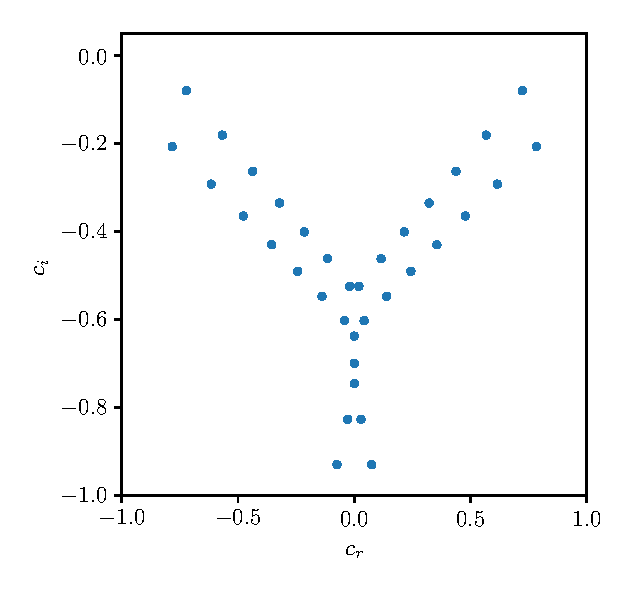
\includegraphics[width=50mm]{figures/c_flow_order_2_3000_M85.eps} \label{subfig:lowMcouette}
    }
    \subfloat[$R = 3000,\ M = 150$]{
        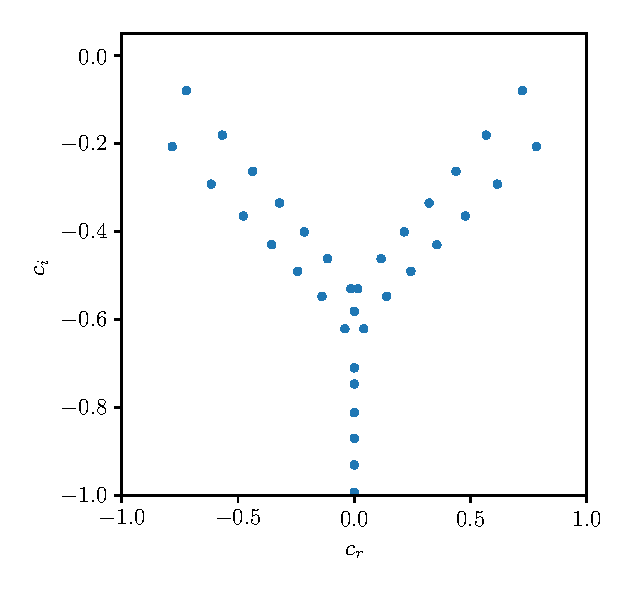
\includegraphics[width=50mm]{figures/c_flow_order_2_3000_M150.eps}
    }
    \subfloat[$R = 3000,\ M = 500 $]{
        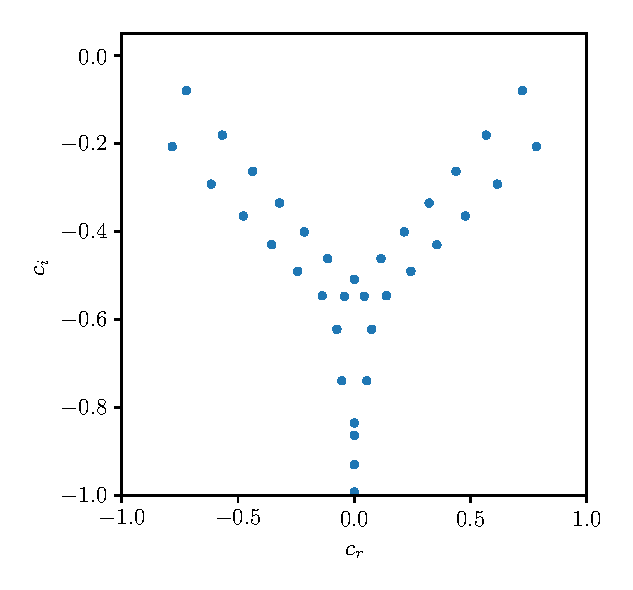
\includegraphics[width=50mm]{figures/c_flow_order_2_3000_M500.eps} \label{subfig:highMcouette}
    }
    \caption{Eigenvalue spectra for various values of $ M $ with $ R = 3000 $}
    \label{fig:couette_inaccdemo}
\end{figure}

This eigenvalue method will always find that Couette flow is stable, which is the expected result \citep{DONGARRA1996399}. This means that there is no 'critical eigenvalue' that we would particularly like to determine and test. We have also already seen in Figure \ref{fig:comparison_couette} that there is a significant difference in the results given based on the order of method used. This indicates that despite its significantly slower computation time, the best method for Couette flow is the first-order method.

\section{Eigenfunction - Poiseuille flow}

One of the key advantages of using the QZ algorithm to solve our system is that we can get the eigenvectors of our system extremely easily, as they are calculated during the process of calculating the eigenvalues \citep{moler1973algorithm}. However, in the case of the first and second-order systems, only the first $ M + 1$ entries correspond to our function $\phi$ and the remaining entries correspond to various derivatives of $\phi$. This means that our eigenfunction is found in this section of the eigenvector.

To get the eigenfunction from this eigenvector recall that the $k$th element corresponds to the coefficient of the $k$th order Chebyshev polynomial. Therefore to calculate our eigenfunction all we have to do is multiply each element by its corresponding Chebyshev polynomial.

Figure \ref{fig:eigenfunction} shows the eigenfunction of the critical mode for plane Poiseuille flow with $ R = 10000$,  $ M = 200 $. In this plot, the eigenfunction has been normalised so that it takes the value $ \phi = 1 + 0i $ at $ z = 0$ as in \citet{thomas1953stability}. The function is symmetric which is expected since the critical mode for plane Poiseuille flow is an even mode. The section of the graph with $ z > 0 $ also looks identical to the graph in \citet{drazin2004hydrodynamic} of the eigenfunction computed by \citet{thomas1953stability}, with one notable difference - the imaginary part is negative in Figure \ref{fig:eigenfunction} whereas, in Drazin and Reid, it is positive. This is because Thomas computed his eigenvalue with a different sign. This also explains why his critical eigenvalue has a negative imaginary part rather than the more common positive imaginary part.

\begin{figure}[h!]
    \centering
    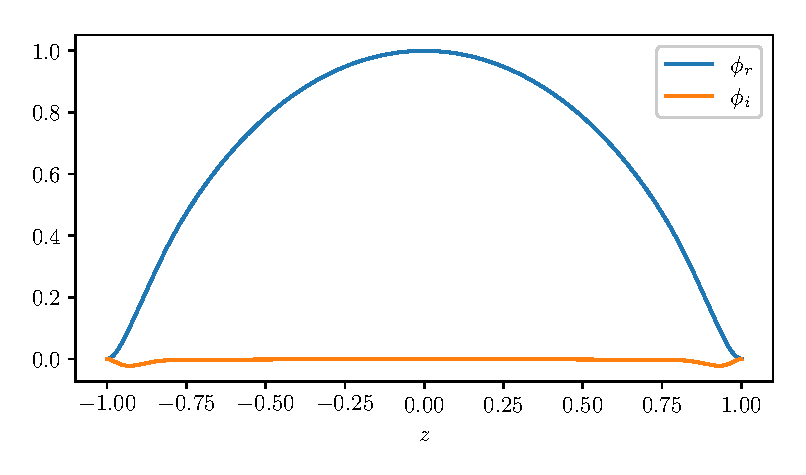
\includegraphics[width=130mm]{figures/eigenfunction.eps}
    \caption{The eigenfunction for the critical mode for plane Poiseuille flow. $ \phi_r $ is the real part and $\phi_i $ is the imaginary part.}
    \label{fig:eigenfunction}
\end{figure}

We can also see that this eigenfunction satisfies the boundary conditions of the Orr-Sommerfeld equation, as it is zero at the boundaries. However, we should also check the derivative of the eigenfunction is zero at the boundaries so that all boundary conditions are satisfied. Using the first order method, all we need to do is to pick the part of the eigenvector corresponding to $ \p_2$ as this is equivalent to $ D \p$. Figure \ref{fig:eigenfunction_diff} shows the plot of this (not normalised). As can be seen, it is zero at the endpoints, showing that all four boundary conditions have been satisfied!

\begin{figure}
    \centering
    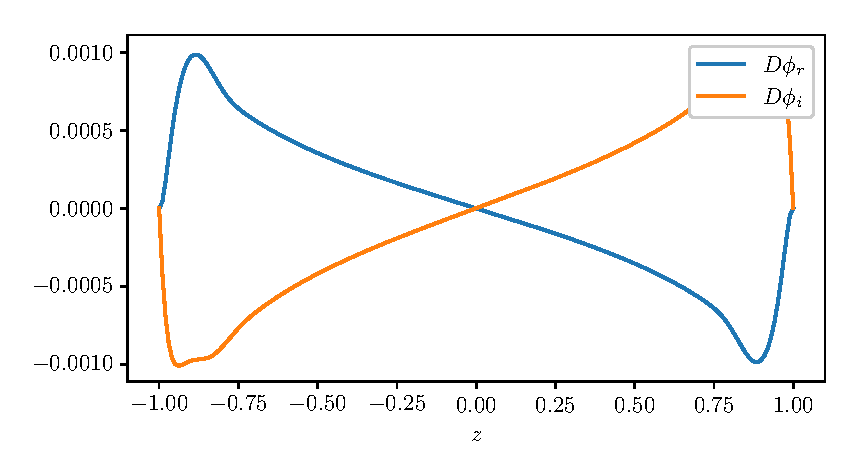
\includegraphics[width=130mm]{figures/eigenfunction_diff.eps}
    \caption{The un-normalized derivative of the eigenfunction for the critical mode of plane Poiseuille flow with $ R = 10000 $ and $ M = 200 $}
    \label{fig:eigenfunction_diff}
\end{figure}

We can take this eigenfunction a little further by computing $ \psi'(z) $, the streamfunction solution we took in Chapter \ref{chap:governing} (equation \eqref{streamfunction}) to get the Orr-Sommerfeld equation. Recall that 
\begin{equation}
    \psi'(x, z, t) = \p(z) \exp{i \alpha (x - c t)},
\end{equation}
where in this case, $ \alpha = 1$ and $ c$ is our critical eigenvalue.

Figure \ref{fig:streamfunction} shows the real part of the streamfunction for the eigenfunction in Figure \ref{fig:eigenfunction} plotted between $ 0 < x < 2 \pi$. As we would expect, it is periodic over this range.

\begin{figure}[h!]
    \centering
    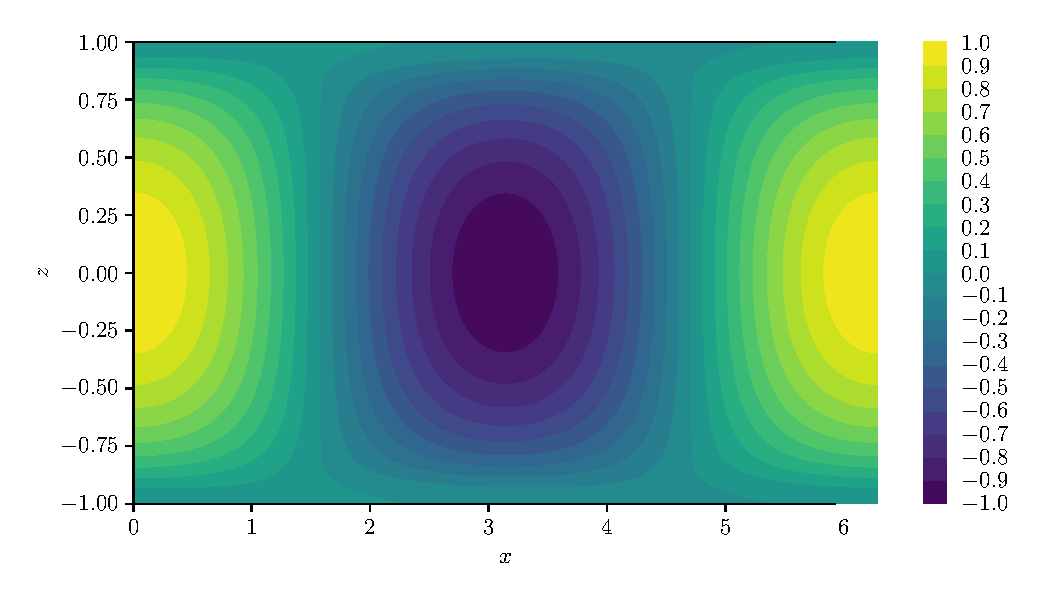
\includegraphics[width=150mm]{figures/streamfunction.eps}
    \caption{The real part of streamfunction for the critical mode of plane Poiseuille flow with $ R = 10000 $ and $ M = 200$}
    \label{fig:streamfunction}
\end{figure}

Code for the eigenfunction plot can be found in Appendix \ref{code:eigenfunction}, and for the streamfunction plot can be found in Appendix \ref{code:streamfunction}.

We can now move on to the most significant result this method can calculate, the critical Reynolds number for Poiseuille flow.

\section{Critical Reynolds Number - Poiseuille flow} \label{section:crit_r}

For a given $ \al$, we can compute the Reynolds number at which the corresponding mode becomes unstable (i.e. the imaginary part of the critical eigenvalue hits $ 0$). We can use this to plot a curve of marginal stability which provides a bound on stability in the same way that the analytic results from \citet{joseph1968eigenvalue, synge1938hydrodynamical} did. The Python program in Appendix \ref{code:criticalR} calculates these values of $ R $ using a bisection technique. The result of this program is shown in Figure \ref{fig:marg_curve}. Notice it takes a very similar shape to Joseph and Synge's bounds, with the unstable $ R$ value appearing to head to infinity as $ \alpha \to 0$ and as $ \alpha \to \infty$. However, the values of $R$ found are much higher than those given by Joseph and Synge. This is likely because the analytic bounds were calculated by significant approximations, and are therefore extremely inaccurate compared to our numerical method.

\begin{figure}[h!]
    \centering
    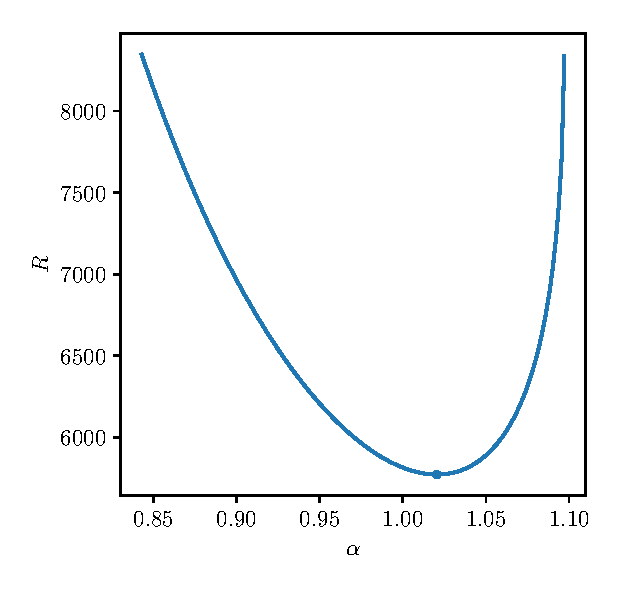
\includegraphics{figures/marginal_stability_curve.eps}
    \caption{The marginal stability curve for Poiseuille flow. The dot indicates the point of critical $R $ and $ \alpha$}
    \label{fig:marg_curve}
\end{figure}

We have a minimum point marked on the graph as a dot. This minimum corresponds to the famous \emph{critical Reynolds number}, the Reynolds number above which Poiseuille flow is unstable. The program computes this by recursively searching for the smallest value near the minimum point. To $6$ significant figures, the first order method with $ 50 $ polynomials finds
\begin{equation}
    R = 5772.22,\ \text{ at } \alpha = 1.02055,
    % R = 5772.221739281689,\ \text{ at } \alpha = 1.0205472421646122
\end{equation}
which matches the findings of \citet{orszag1971accurate}, who found that the first unstable mode of plane Poiseuille flow occurs at $ R = 5772.2 $ with $ \alpha = 1.02056 \pm 0.00001 $.

A value for the critical Reynolds number for Couette flow does exist, at about $ R = 45000 $ \citep{bukhari1997spectral}. Unfortunately, we cannot reproduce this value using this program as accuracy is lost so fast as $ R $ increases with Couette flow. Interestingly, \citet{bukhari1997spectral} quotes a slightly lower value for plane Poiseuille flow, although this doesn't seem to be supported in other literature, and our program cannot reproduce this value either.

These results differ significantly from those predicted by our analytic bounds from Chapter \ref{chap:suffcons}. The critical Reynolds number computed numerically is much higher for Poiseuille flow than the value obtained analytically. Recall that Joseph's more accurate bound predicted a value of roughly $ 9 $! However, Joseph and Synge's bounds did expect that the critical Reynolds number would be found at a low wavenumber, which we have found to be the case.

% \section{Basic Results - Poiseuille Flow}
% We first run the $2$nd order method for Poiseuille flow using the standard differentiation matrices suggested by \citet{dongarra1996chebyshev} for $ \al = 1, R = 10000 $ with $ 200 $ polynomials. This produces the classic eigenvalue spectra for plane Poiseuille flow found in many papers.

% The spectra can be seen in Figure \ref{fig:r10000} and forms a 'Y' shape. We can see that there are 3 distinct 'families' of eigenvalues \citep{mack1976numerical}. The bottom straight line is referred to as the S family and contains a pattern of alternating odd and even eigenvalues \citep{dongarra1996chebyshev}, the top right branch is referred to as the P family and consists of overlapping pairs of odd and even eigenvalues \citep{dongarra1996chebyshev} and the 'spray' of eigenvalues forming the left branch is referred to as the A family of eigenvalues.
% \begin{figure}[h!]
%     \centering
%     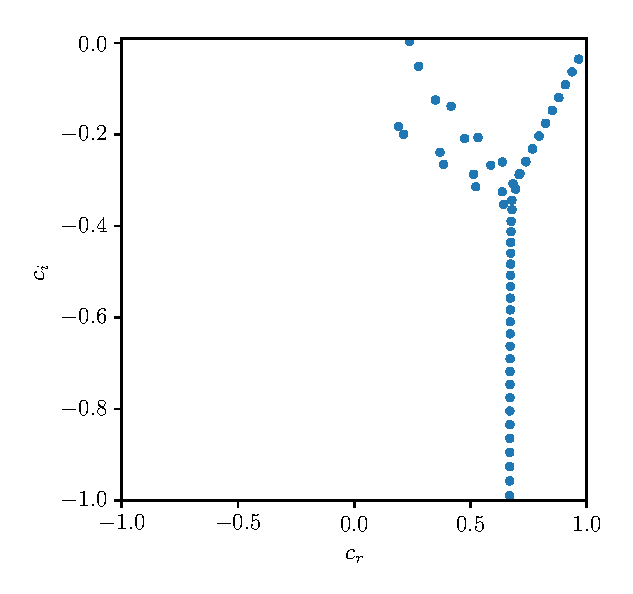
\includegraphics{figures/D2methodbig10000.eps}
%     \caption{Eigenvalue spectra for plane Poiseuille flow with $ \al = 1 $ and $ R = 10000 $}
%     \label{fig:r10000}
% \end{figure}

% We aim to reproduce the graphs seen in \citet{bukhari1997spectral} for the $ D^2 $ method. These all use $ \al = 1 $, $ 200 $ polynomials and $ R $ values between $ 5000 $ and $ 50000 $. We also include a graph of $ R = 100 $ and compare it to the graph found in \citet{antar1976eigenvalue}. 

% Note that the graph in \citet{antar1976eigenvalue} includes only the eigenvalues corresponding to the symmetric (even) modes (our program provides all the eigenvalues within the given range) and also that this graph has different limits on $ c_i $ to the other graphs.

% The spectra produced by our program can be seen in Figure \ref{fig:pspectra}. As can be seen, they match exactly with the graphs found in \citet{bukhari1997spectral, antar1976eigenvalue}. However, there is some interesting behaviour in the $ R = 30000 $ and $ R = 50000 $ cases. This is caused by either too few polynomials or numerical error and will be the focus of the next section where we analyse the accuracy of our various methods.
% \begin{figure}[p!]
%     \centering
%     \subfloat[$\al = 1 $ with $ R = 100 $]{
%         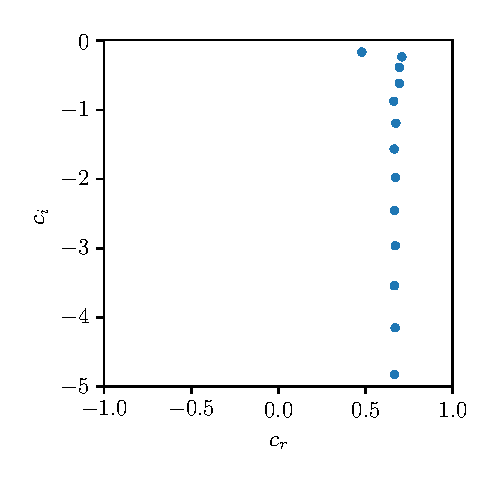
\includegraphics{figures/D2method100.eps}
%     }
%     \subfloat[$\al = 1 $ with $ R = 5000 $]{
%         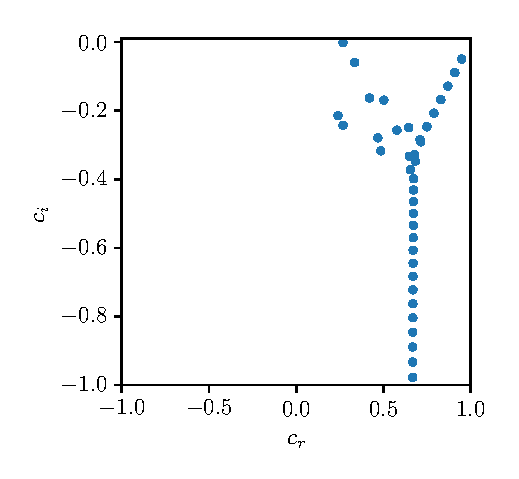
\includegraphics{figures/D2method5000.eps}
%     }
%     \hspace{0mm}
%     \subfloat[$\al = 1 $ with $ R = 7500 $]{
%         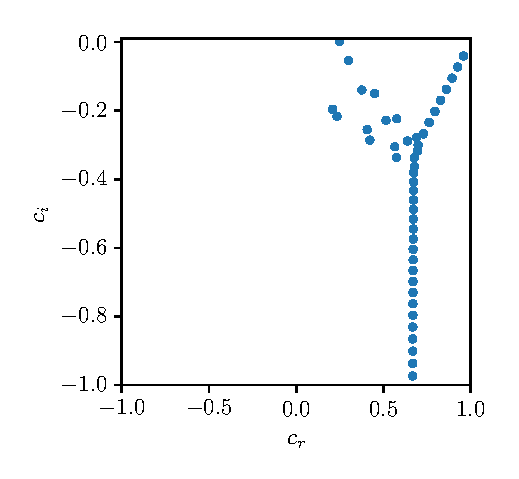
\includegraphics{figures/D2method7500.eps}
%     }
%     \subfloat[$\al = 1 $ with $ R = 10000 $]{
%         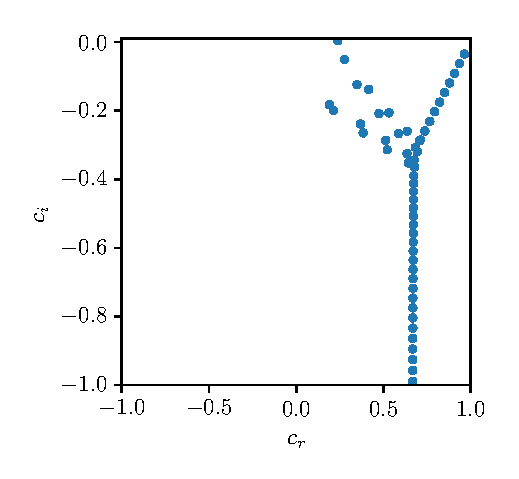
\includegraphics{figures/D2method10000.eps}
%     }
%     \hspace{0mm}
%     \subfloat[$\al = 1 $ with $ R = 30000 $]{
%         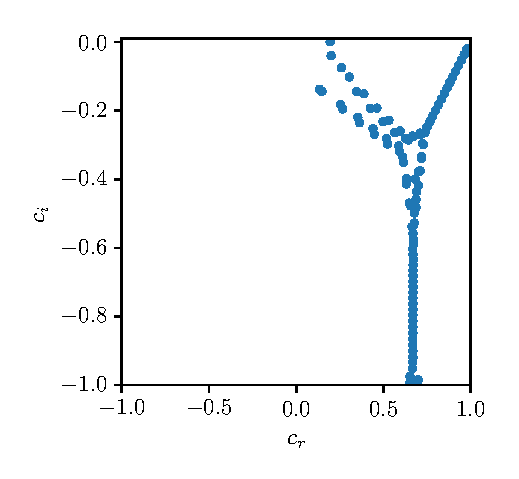
\includegraphics{figures/D2method30000.eps}
%     }
%     \subfloat[$\al = 1 $ with $ R = 50000 $]{
%         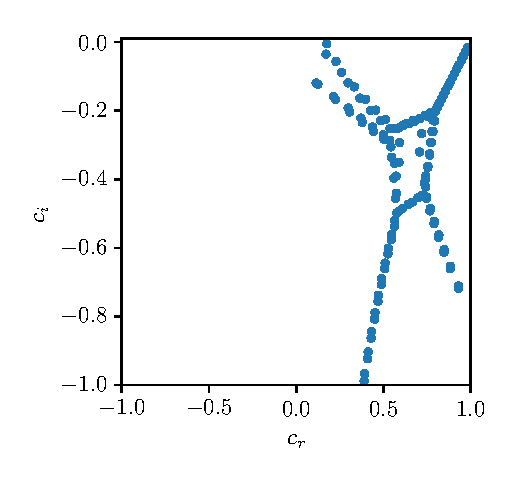
\includegraphics{figures/D2method50000.eps}
%     }
%     \caption{Graphs of the eigenvalue spectra for Poiseuille flow with $ \al = 1 $ and various values of $ R $}
%     \label{fig:pspectra}
% \end{figure}

% \textbf{discuss what values of polynomials are needed for this value to be found, e.g. for the 4th order case we cannot get the exact value as found by orszag} 

% \section{Basic Results - Couette Flow}

% \textbf{Show graphs of spectra}



% \section{Comparison and accuracy of methods}
% First we would like to compare the accuracy of our 4 different methods. To start we will examine the accuracy of just one method, the standard $2$nd order method. 

% Compare numerical accuracy, plots as in \cite{dongarra1996chebyshev} (triangle of numerical instability)

% Compare D4, D2, D1 methods. Compare both Poiseuille and Couette flow

% Plot curves of error for critical eigenvalue - a little cruder than some papers as Python returns eigenvalues in random order

% \textbf{comparision of time taken}

% \begin{figure}
%     \centering
%     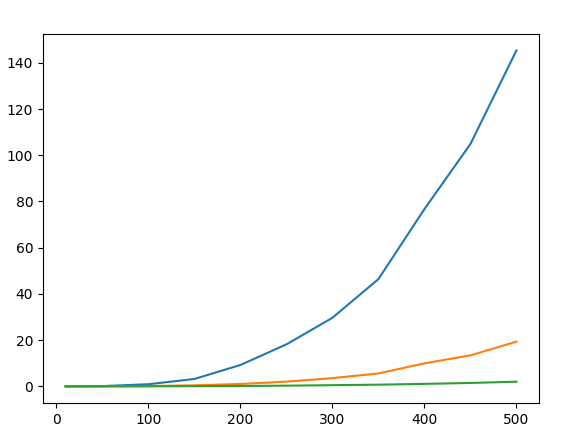
\includegraphics{figures/timecomp.png}
%     \caption{A comparison of time taken for various values of $M$ - PLACEHOLDER}
%     \label{fig:time_comp}
% \end{figure}


% \section{Critical Reynolds Number}

% curve of marginal stability
% compute for poiseuille and couette (if possible for couette)

% \section{Eigenfunction}

% Normalized the value at 0 to be $ 1 + 0 i $ as in \cite{thomas1953stability}, produces graph seen in \cite{drazin2004hydrodynamic}

% The program correctly produces an even eigenfunction, which is what we would expect

% % \section{Reynold's stress tensor}
% % As in \cite{drazin2004hydrodynamic}, \cite{stuart1966double}

% % \section{Stabilizing Poiseuille flow with Couette flow}
% % As \cite{potter1966stability, hains1967stability, reynolds1967finite}  